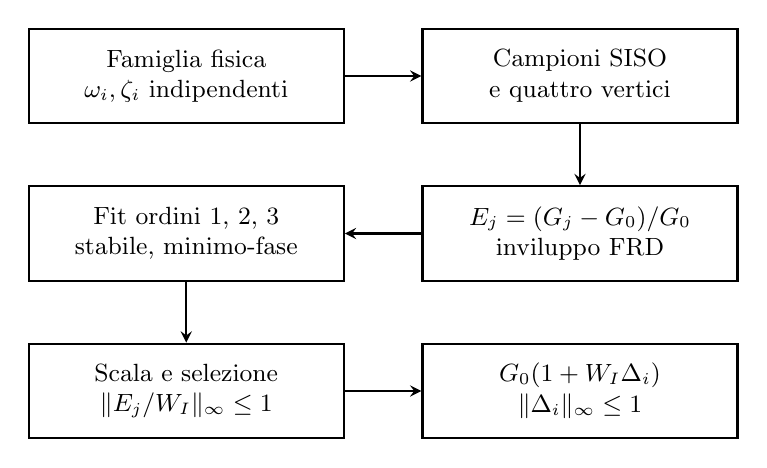
\begin{tikzpicture}[>=stealth,thick,every node/.style={font=\small},box/.style={draw,align=center,minimum width=40mm,minimum height=12mm}]
\node[box] (a) at (0,0) {Famiglia fisica\\$\omega_i,\zeta_i$ indipendenti};
\node[box] (b) at (5,0) {Campioni SISO\\e quattro vertici};
\node[box] (c) at (5,-2) {$E_j=(G_j-G_0)/G_0$\\inviluppo FRD};
\node[box] (d) at (0,-2) {Fit ordini 1, 2, 3\\stabile, minimo-fase};
\node[box] (e) at (0,-4) {Scala e selezione\\$\|E_j/W_I\|_\infty\leq1$};
\node[box] (f) at (5,-4) {$G_0(1+W_I\Delta_i)$\\$\|\Delta_i\|_\infty\leq1$};
\draw[->](a)--(b);\draw[->](b)--(c);\draw[->](c)--(d);\draw[->](d)--(e);\draw[->](e)--(f);
\end{tikzpicture}
